\chapter{Models}\label{final}

\section{Artificial Neural Network(ANN)}
Artificial Neural Networks are a special type of machine learning algorithms that are modeled after the human brain. That is, just like how the neurons in our nervous system are able to learn from the past data, similarly, the ANN is able to learn from the data and provide responses in the form of predictions or classifications.ANNs are nonlinear statistical models which display a complex relationship between the inputs and outputs to discover a new pattern.\cite{models}
 In a neural network, there are three essential layers –
 \begin{itemize}
     \item  Input Layer- It is the first layer of an ANN that receives the input information in the form of various texts, numbers, audio files, image pixels, etc.
     \item Hidden Layer - In the middle of the ANN model are the hidden layers. There can be a single hidden layer, as in the case of a perceptron or multiple hidden layers. These hidden layers perform various types of mathematical computation on the input data and recognize the patterns that are part of.
     \item Outer Layer -In the output layer, we obtain the result that we obtain through rigorous computations performed by the middle layer.
 \end{itemize}
 
 \begin{figure}
\makebox[\textwidth][c]{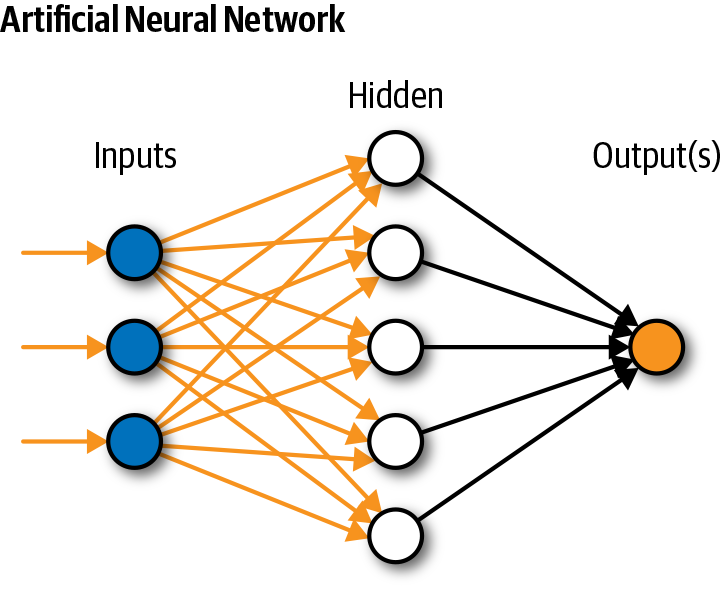
\includegraphics[width=0.6\textwidth]{others/ann.png}}%
  \caption{ANN}
  \label{fig:key}
\end{figure}
\section{Recurrent neural network(RNN)}
A recurrent neural network is a class of artificial neural networks where connections between nodes form a directed graph along a temporal sequence. This allows it to exhibit temporal dynamic behavior.It is derived from feedforward neural networks, RNNs can use their internal state (memory) to process variable length sequences of inputs.The term “recurrent neural network” is used indiscriminately to refer to two broad classes of networks with a similar general structure, where one is finite impulse and the other is infinite impulse. Both classes of networks exhibit temporal dynamic behavior.Both finite impulse and infinite impulse recurrent networks can have additional stored states, and the storage can be under direct control by the neural network. The storage can also be replaced by another network or graph, if that incorporates time delays or has feedback loops.\cite{rnn}
\begin{figure}
\makebox[\textwidth][c]{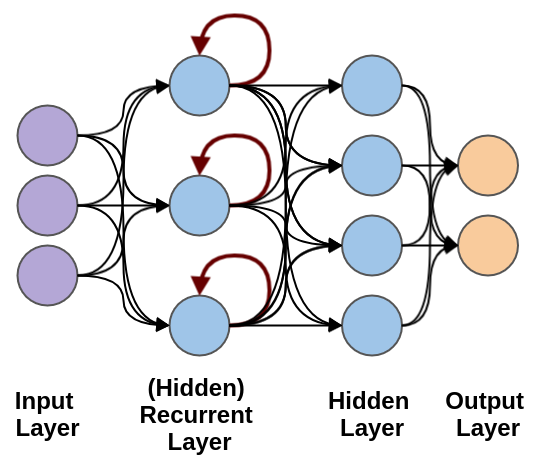
\includegraphics[width=0.6\textwidth]{others/rnn-multihidden.png}}%
  \caption{Recurrent neural network}
  \label{fig:key}
\end{figure}
\section{Long short-term memory (LSTM) }
Long Short-Term Memory (LSTM) networks are a type of recurrent neural network capable of learning order dependence in sequence prediction problems.LSTMs have the  ability to preserve long-term memory and  have a slightly more complex structure. At each time step, the LSTM cell takes in 3 different pieces of information -- the current input data, the short-term memory from the previous cell (similar to hidden states in RNNs) and lastly the long-term memory.The short-term memory is commonly referred to as the hidden state, and the long-term memory is usually known as the cell state.The cell then uses gates to regulate the information to be kept or discarded at each time step before passing on the long-term and short-term information to the next cell.These gates are called the Input Gate, the Forget Gate, and the Output Gate.\cite{lstm}
\begin{figure}
\makebox[\textwidth][c]{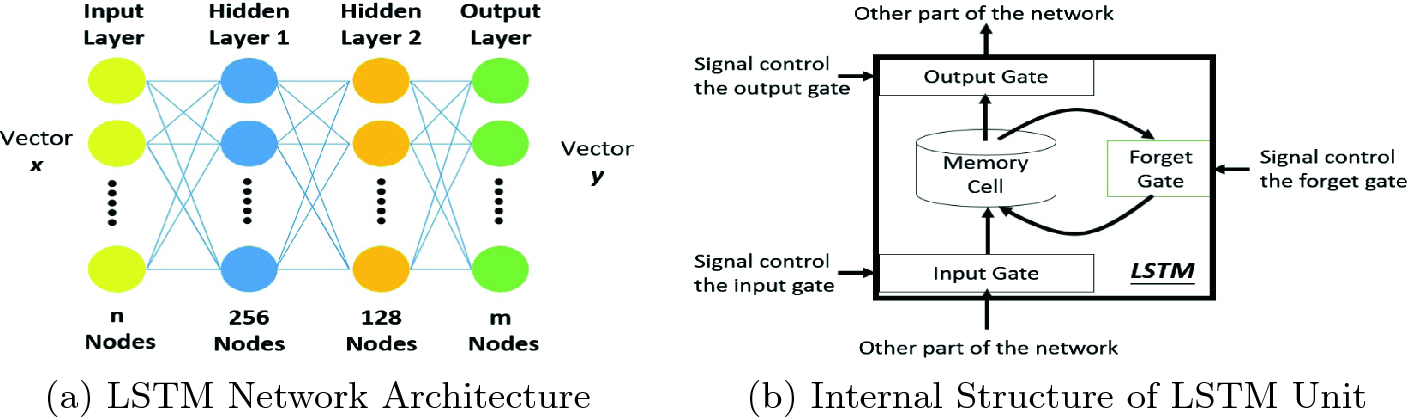
\includegraphics[width=1.2\textwidth]{others/lstm.png}}%
  \caption{LSTM}
  \label{fig:key}
\end{figure}
\section{ Gated Recurrent Unit(GRU)}
A Gated Recurrent Unit is a variant of the RNN architecture, and uses gating mechanisms to control and manage the flow of information between cells in the neural network.The structure of the GRU allows it to adaptively capture dependencies from large sequences of data without discarding information from earlier parts of the sequence. This is achieved through its gating units, similar to the ones in LSTMs, which solve the vanishing gradient problem of traditional RNNs. These gates are responsible for regulating the information to be kept or discarded at each time step.The GRU cell contains only two gates: the Update gate and the Reset gate.These gates in the GRU are trained to selectively filter out any irrelevant information while keeping what’s useful. These gates are essentially vectors containing values between 0 to 1 which will be multiplied with the input data and/or hidden state.
A 0 value in the gate vectors indicates that the corresponding data in the input or hidden state is unimportant and will, therefore, return as a zero. On the other hand, a 1 value in the gate vector means that the corresponding data is important and will be used.
\begin{figure}
\makebox[\textwidth][c]{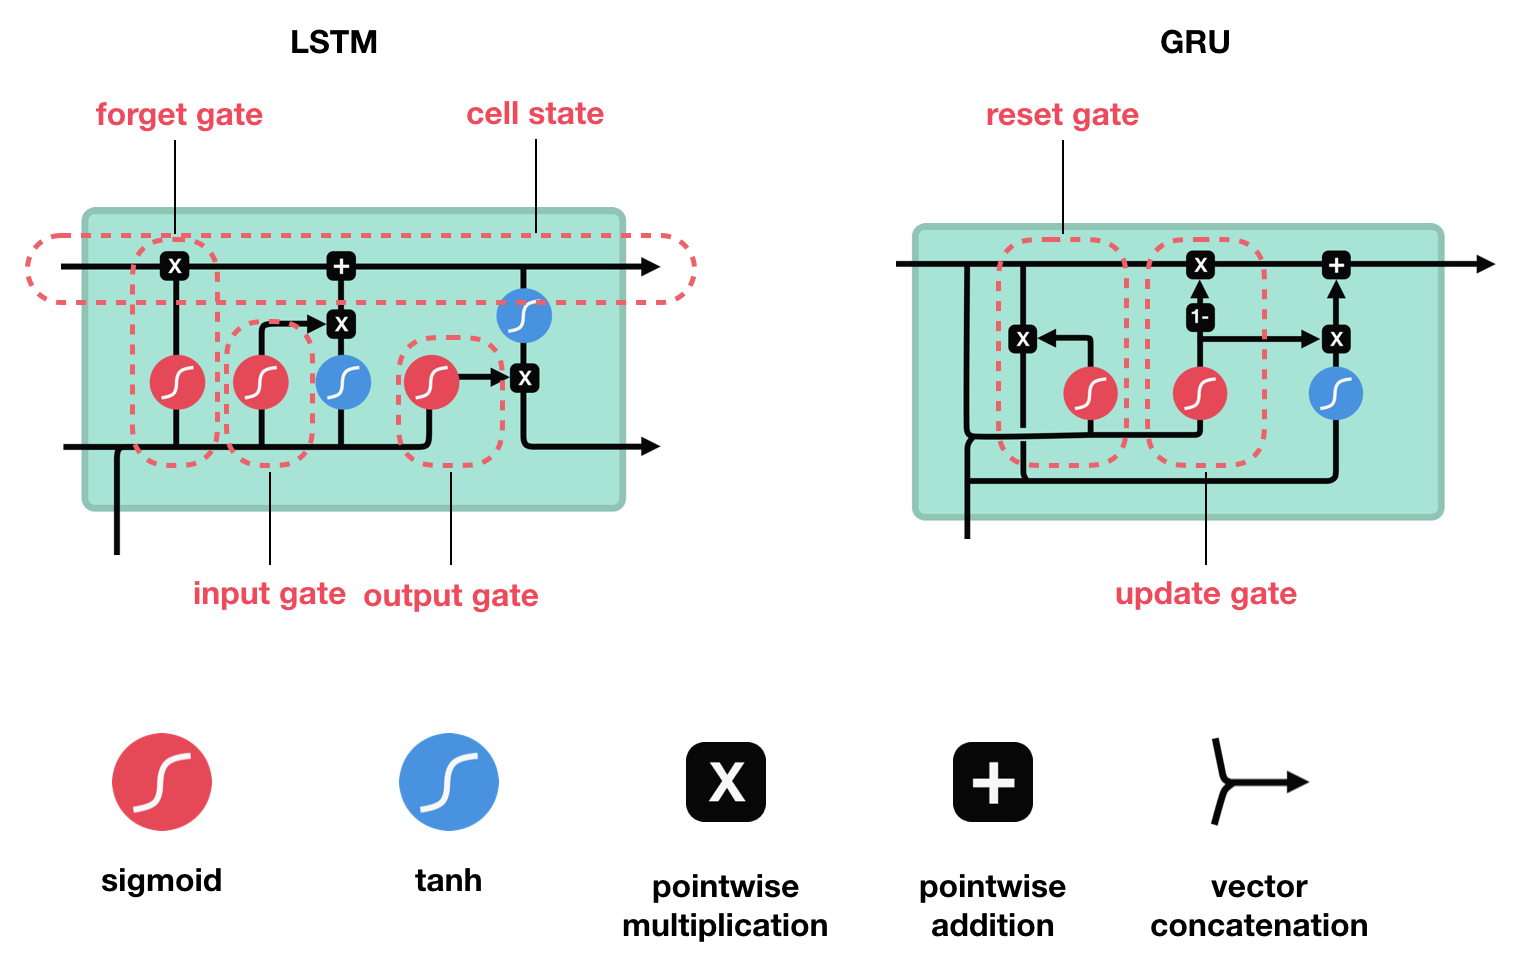
\includegraphics[width=0.8\textwidth]{others/gru.png}}%
  \caption{LSTM vs GRU}
  \label{fig:key}
\end{figure}
\section{ Convolutional Neural Network (CNN)}
In deep learning, a convolutional neural network (CNN, or ConvNet) is a class of deep neural network, most commonly applied to analyze visual imagery
We track sizes of communities across time.
As the community labels are changing, we keep track of size changes by cluster memberships.CNNs are regularized versions of multilayer perceptrons. Multilayer perceptrons usually mean fully connected networks, that is, each neuron in one layer is connected to all neurons in the next layer.A convolutional neural network consists of an input layer, hidden layers and an output layer. In any feed-forward neural network, any middle layers are called hidden because their inputs and outputs are masked by the activation function and final convolution. In a convolutional neural network, the hidden layers include layers that perform convolutions. \cite{cnn}

\begin{figure}
\makebox[\textwidth][c]{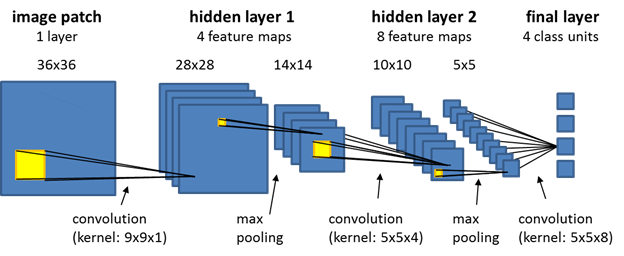
\includegraphics[width=0.8\textwidth]{others/cnn.png}}%
  \caption{CNN}
  \label{fig:key}
\end{figure}


\section{Isolation Forest}
Isolation forest is an unsupervised learning algorithm for anomaly detection that works on the principle of isolating anomalies,instead of the most common techniques of profiling normal points.An anomaly is an observation or event that deviates so much from other events to arouse suspicion it was generated by a different mean.Anomalies in a big dataset may follow very complicated patterns, which are difficult to detect “by eye” in the great majority of cases.In order to isolate a data point(outlier), the algorithm recursively generates partitions on the sample by randomly selecting an attribute and then randomly selecting a split value for the attribute, between the minimum and maximum values allowed for that attribute.\cite{isolationF}
\begin{figure}
\makebox[\textwidth][c]{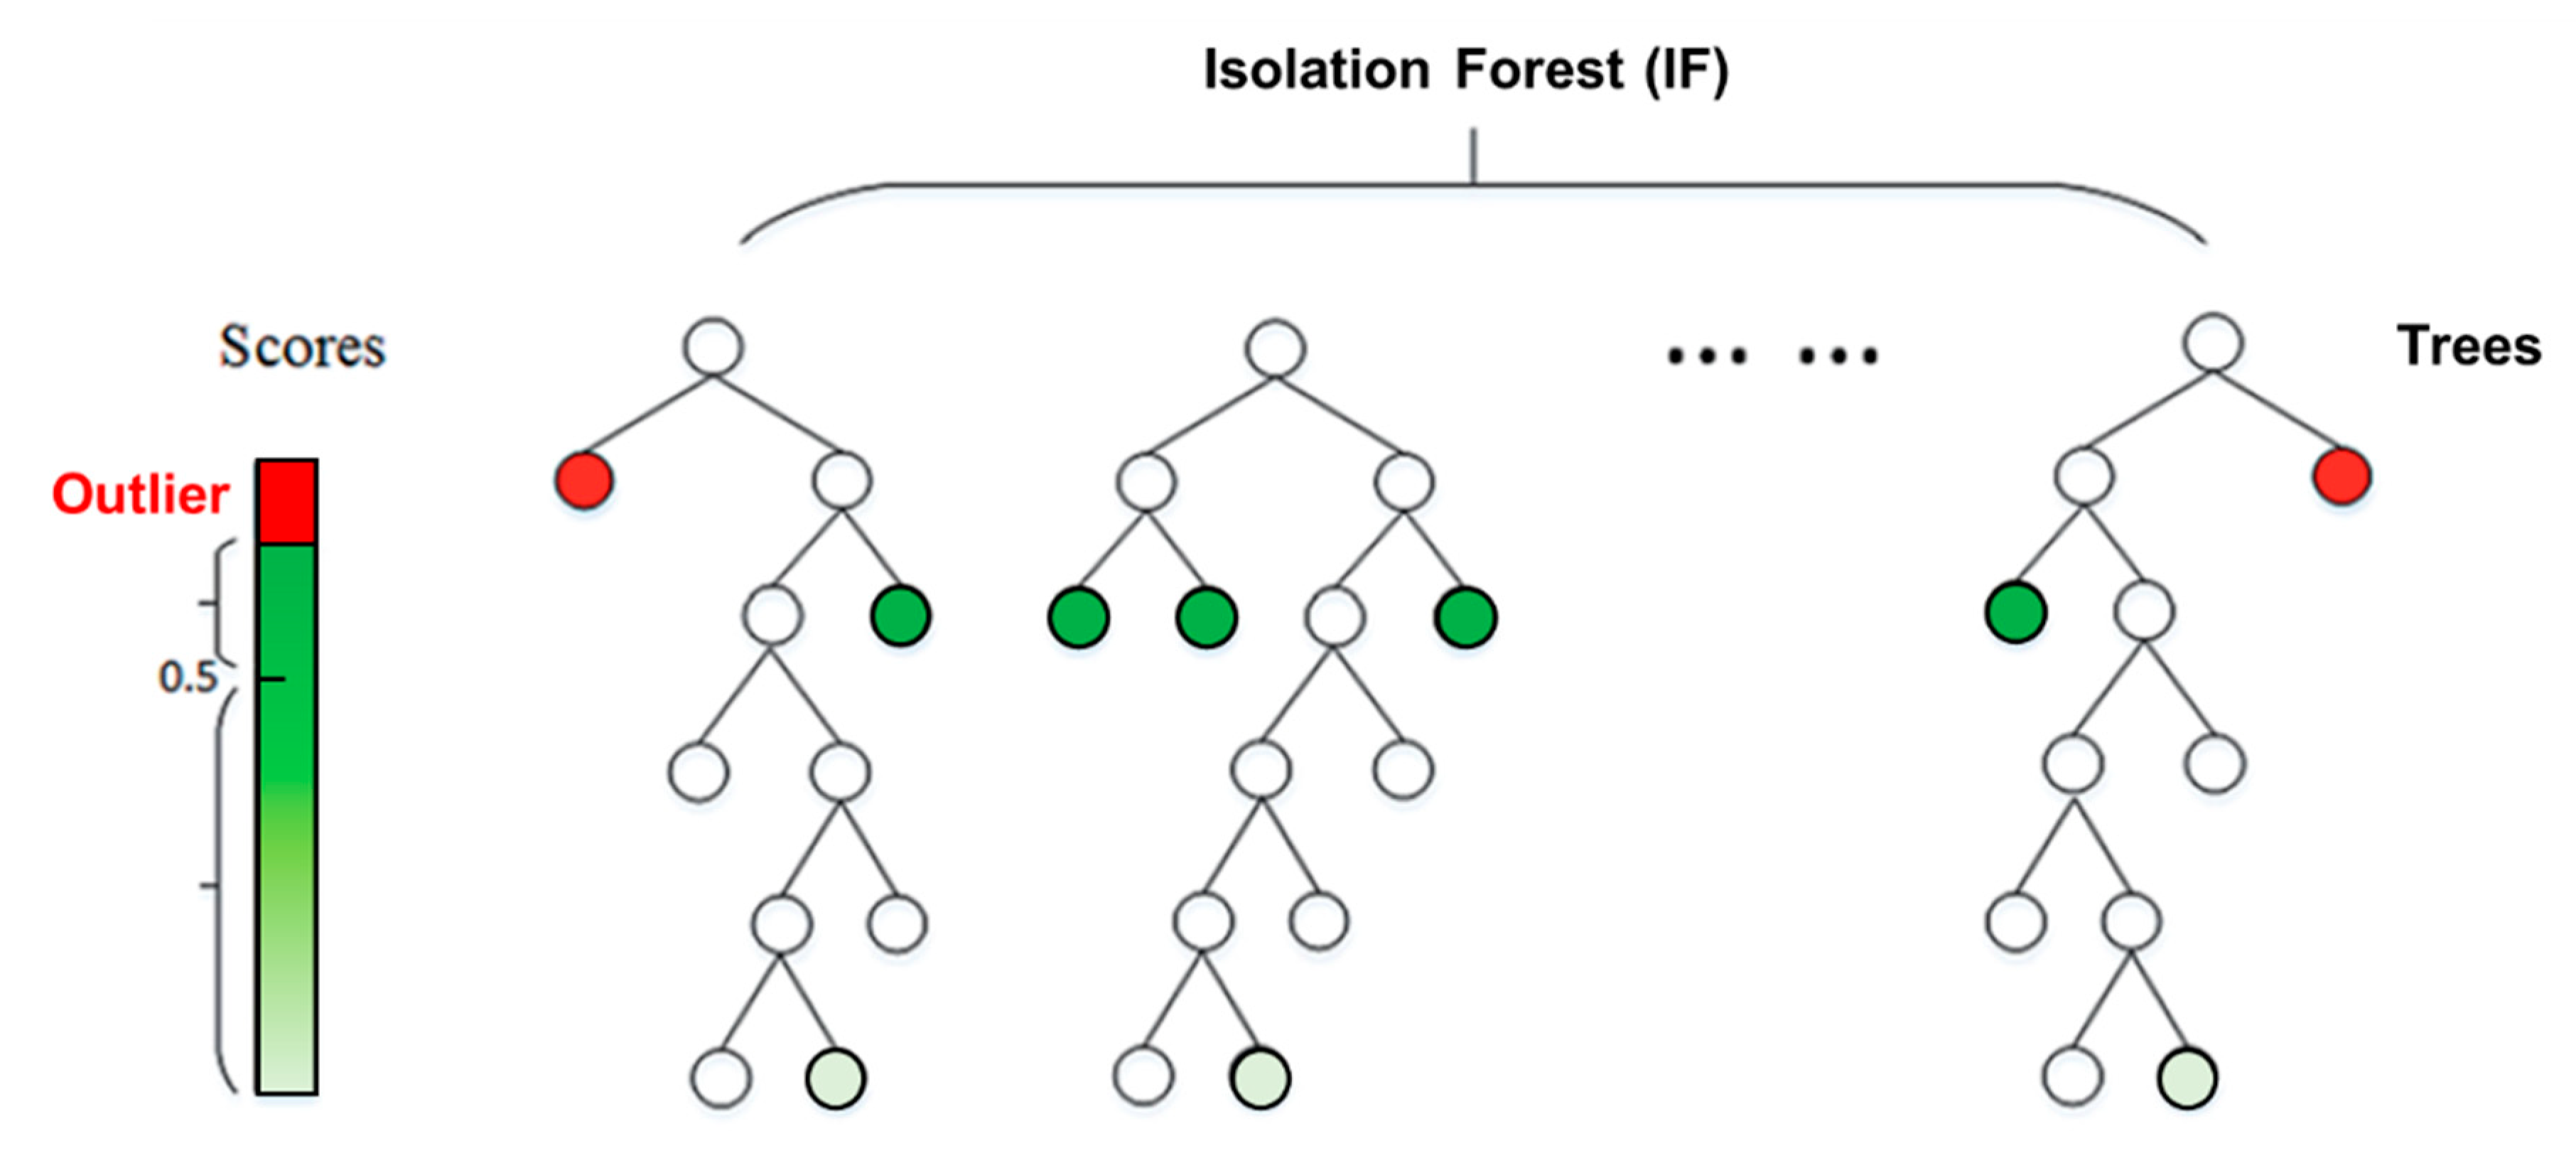
\includegraphics[width=0.8\textwidth]{others/isolation.png}}%
  \caption{Isolation Forest}
  \label{fig:key}
\end{figure}





 